\section{Principes de DICOM}

	\frame
	{
		\frametitle{Objectifs globaux}
		\begin{itemize}
			\item<1-> Trouver un langage commun pour l'\'echange (images et donn\'ees pertinentes) entre \'equipements d'imagerie : mettre en place un standard.
			\item<2-> Pousser les vendeurs \`a parler et comprendre ce langage commun.
			\item<3-> Standardiser :
			\begin{itemize}
				\item<4-> le stockage (i.e. format de fichier) ;
				\item<5-> et la communication des donn\'es (i.e. protocoles de communication).
			\end{itemize}
		\end{itemize}
	}
	
	\frame
	{
		\frametitle{Objectifs sp\'ecifiques}
		
        Il faut que lors de l'installation d'une nouvelle modalit\'e, le DICOM permette, sans changement d'un quelconque composant logiciel (\emph{i.e.~Plug~\&~Play}) :
		\begin{itemize}
			\item<1-> l'interrogation du PACS ;
			\item<2-> la r\'ecup\'eration des images cr\'e\'ees par d'autres syst\`emes ;
			\item<3-> l'affichage des images ;
			\item<4-> et la production d'images lisibles par les syst\`emes d'autres constructeurs.
		\end{itemize}
	}

	\frame
	{
		\frametitle{Prescription d'un examen radiologique}
		\begin{itemize}
			\item Sch\'ematisation de la proc\'edure :
			%\includegraphics<2->[width=\linewidth]{./figures/scenario-1.png}
			%\includegraphics<3->[width=\linewidth]{./figures/scenario-2.png}
			%\includegraphics<4->[width=\linewidth]{./figures/scenario-3.png}
			%\includegraphics<5->[width=\linewidth]{./figures/scenario-4.png}
			%\includegraphics<6->[width=\linewidth]{./figures/scenario-5.png}
			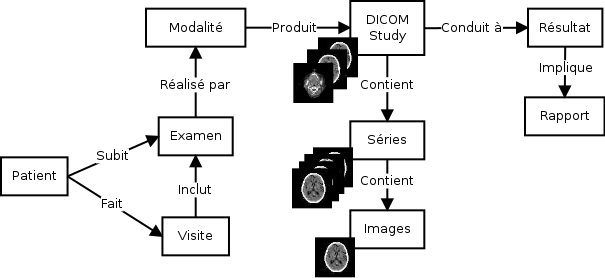
\includegraphics[width=\linewidth]{./figures/scenario.png}
			\item<2-> DICOM d\'ecrit ces donn\'ees et ces relations.
			\item<3-> La pr\'ecision du contenu et des liens d\'epend des outils et des utilisateurs (\emph{e.g.} RIS, PACS).
		\end{itemize}
	}

	\frame
	{
		\frametitle{Traduire le r\'eel en num\'erique}
		
		\begin{itemize}
			\item Un objet DICOM combine :
			\begin{itemize}
				\item<2-> des donn\'ees, ou informations (e.g. un patient, une image, \ldots)
				\begin{itemize}
					\item<3-> contenues dans un \emph{Information Object},
					\item<4-> d\'efini dans la norme par une \emph{Information Object Definition} (ou \emph{IOD}) ;
				\end{itemize}
				
				\item<5-> et une fonction pr\'ecise (e.g. stocker, imprimer,\ldots)
				\begin{itemize}
					\item<6-> c'est-\`a-dire un \emph{Service},
					\item<7-> d\'efini par un \emph{DICOM Message Service Element} (ou \emph{DIMSE})
				\end{itemize}
			\end{itemize}
			\item<8-> Une norme doit lister toutes les combinaisons possibles.
		\end{itemize}
	}
	
	\frame
	{
		\frametitle{Un identifiant unique : le SOP Class UID}

		\begin{itemize}
			\item La combinaison Information Object + Service est :
			\begin{itemize}
				\item<2-> appel\'ee \emph{Service/Object Pair} (ou \emph{SOP}) ;
				\item<3-> un \'el\'ement important pour d\'eterminer la conformit\'e � la norme ;
				\item<4-> identifi\'ee par un identifiant unique nomm\'e \emph{SOP Class UID}.
			\end{itemize}
		
			\item<5-> Norme DICOM = annuaire de SOP.\\
			SOP Class UID (identifiant unique d'un type de paire service/objet) = num\'ero unique pour trouver \`a quelle paire Service/Objet correspond un objet.
			\item<6-> Analogie : annuaire\\
			Un num\' ero = paire \{nom $+$ adresse\}.
			\item<7-> Exemples de SOP Class UID :
			\begin{description}
				\item<8->[$1.2.840.10008.5.1.4.1.1.1$] CR Image Store (enregistrer un CR) ;
				\item<9->[$1.2.840.10008.5.1.4.1.1.2$] CT Image Store (enregistrer un CT).
			\end{description}
		\end{itemize}
	}
	
	\frame
	{
		\frametitle{Sch\'ema de construction du SOP}
		\begin{center}
			\includegraphics<1>[width=\linewidth]{./figures/sop-definition.png}
			\includegraphics<2>[width=\linewidth]{./figures/sop-definition-IOD.png}
		\end{center}		
	}

